\documentclass[times, utf8, seminar]{fit}

%\batchmode
%\usepackage{booktabs}
\usepackage{listings}
\usepackage{longtable}
\usepackage{xcolor}
\usepackage{float}
\usepackage{enumitem}
\usepackage{hyperref}
\usepackage{enumerate}
\usepackage{graphicx}
\usepackage{etoolbox}
\usepackage{datetime}
\usepackage{needspace}
\usepackage{titlesec}
%\titleformat{\chapter}[display]{\normalfont\huge\bfseries}{\chaptertitlename\ \thechapter}{20pt}{\Huge}

\begin{document}
\widowpenalty=300
\clubpenalty=300

\lstset{
  language=bash,
  backgroundcolor=\color{gray!25},
  basicstyle=\ttfamily \footnotesize,
  breaklines=true,
  prebreak=\raisebox{0ex}[0ex][0ex] \hookleftarrow,
  columns=fullflexible
}


% this alters "before" spacing (the second length argument) to 0
%\titlespacing*{\chapter}{0pt}{0pt}{40pt}

% this changes "before" spacing back to its default of 50pt
%\titlespacing*{\chapter}{0pt}{50pt}{40pt}}

%\titlespacing*{\chapter}{0pt}{-50pt}{18pt}
%\titleformat{\chapter}[display]{\normalfont\huge\bfseries}{\chaptertitlename\ \thechapter}{20pt}{\Huge}

\title{Agilni \em{software development},\newline GIT SCM}

\author{Ernad Husremović}
\brindex{DL 2792}
\verzija {0.0.1}

\mentor{mr. Adil Joldić}

\maketitle

\tableofcontents

%\listoftables
%\listoffigures
\newpage

\begin{abstract}

Dokument na bazi konkretnog primjera (`HOWTO' stil) objašnjava uobičajeni developerski `workflow' pri korištenu GIT SCM-a. U promjeru se koriste GIT Web servisi `Github' i `Gitlab'.
Čitalac bi čitanjem materijala trebao upoznati osnovne operacije GIT klijenta kao i navedenih Web servisa.


\keywords{open source software, OSS, Source code management, SCM, DSCM, Version control, GIT}
\end{abstract}

% abstract end

\chapter{Uvod}
\vspace*{-0.7cm}

\section{`Source code management' (SCM) software}

`Source code management' (SCM) software obezbjeđuje pohranu različitih verzija programskog koda u zajednički repozitorij. 
Iako je prvobitna ovih alata bilo čuvanje programskog koda, oni se mogu koriste za za pohranu (verzioniranje) svih artifakta softverskog projekta uključujući dokumentaciju, dijagrame, binarni kod.
Ovaj software se često naziva i `Version control' software.

Sa stanovišta arhitekture, SCM sistemi se dijele na centralizovane i distribuirane (DSCM).

\subsection{Centralizirani (mrežni) SCM}

Najpoznatiji predstavnici su `CVS' i `Subversion'. `CVS' je među prvim SCM alatima-ima koji je postigao veliku popularnost.

`Subversion' je uveo značajna tehnička unapređenja, ali je arhitekturalno identičan svom predhodniku. Oba alata su `open source' software (OSS).

Njihova glavna karakakteristika je klasična `client-server' arhitektura. Da bi se SCM operacije na klijentu izvršavale, neophodna je dostupnost SCM servera.
Razlog je taj što se istorija promejan nalazi isključivo na serveru.

Ova karakteristika danas se smatra ključnim nedostatkom centraliziranih SCM-ova

\subsection{Distribuirani SCM (DSCM)}

Distribuirani SCM-omi imaju potpuno različitu arhitekturu. Baza promjena nalazi se na svakom klijentu.
Sami developeri određuju funkciju pojedinačnih repozitorija. Glavni repozitorij (`upstream') je dostupan udaljenim klijentima.
Razmjena podataka (`commit'-a) se vrši sistemom sinhronizacije repozitorija klijenta i servera (`merge' proces). 
Usljed nedostatka centralnog repozitorija, sasvim su normalne situacije u kojima se repozitoriji koji se usaglašavaju - sinhronizuju u stanju konflikta.
U tom slučaju potrebno je izvršiti manuelni `merge` proces kojim se promjene primljene iz različitih izvora usaglašavaju.
Iako ovaj koncept na prvi pogled djeluje kao izvor velikih glavobolja, pravilna primjena DSCM alatima daje veliku fleksibilnost i niz prednosti u odnosu na centralizirane SCM-ove.

Jedna od ključnih prednosti DSM-ova je `off-line' režim rada, kao posljedica činjenice da svaki korisnik ima sopstveni lokalni repozitorij promjena.

\chapter{Gitlab servis}
\vspace*{-0.7cm}

\begin{figure}[H]
\centering
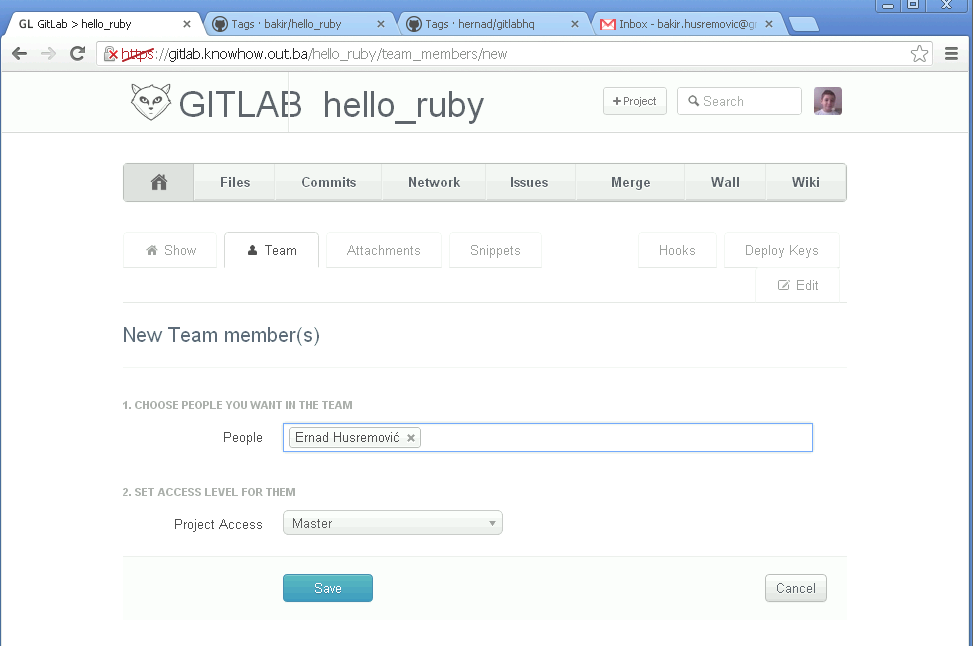
\includegraphics[width=15cm]{img/gitlab_add_new_member_to_project.png}
\caption{Gitlab dodaj novog člana u projekat}
\end{figure}


\begin{figure}[H]
\centering
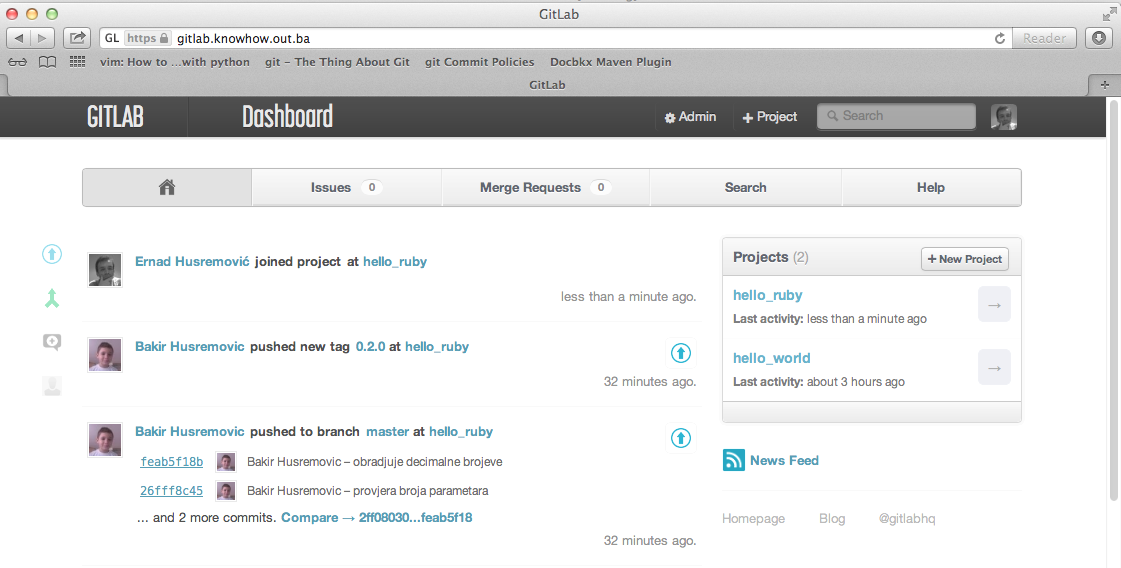
\includegraphics[width=15cm]{img/gitlab_add_new_member_to_project_2.png}
\caption{Gitlab dodaj novog člana u projekat 2}
\end{figure}

\section{Github servis}

\begin{figure}[H]
\centering
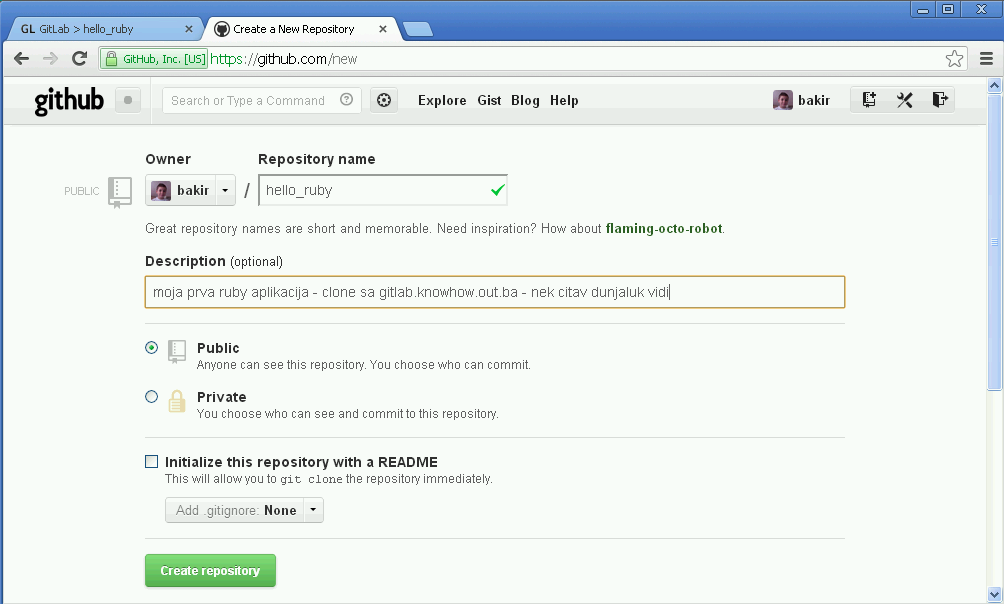
\includegraphics[width=15cm]{img/github_new_repos.png}
\caption{Github novi repozitorij}
\end{figure}

\begin{figure}[H]
\centering
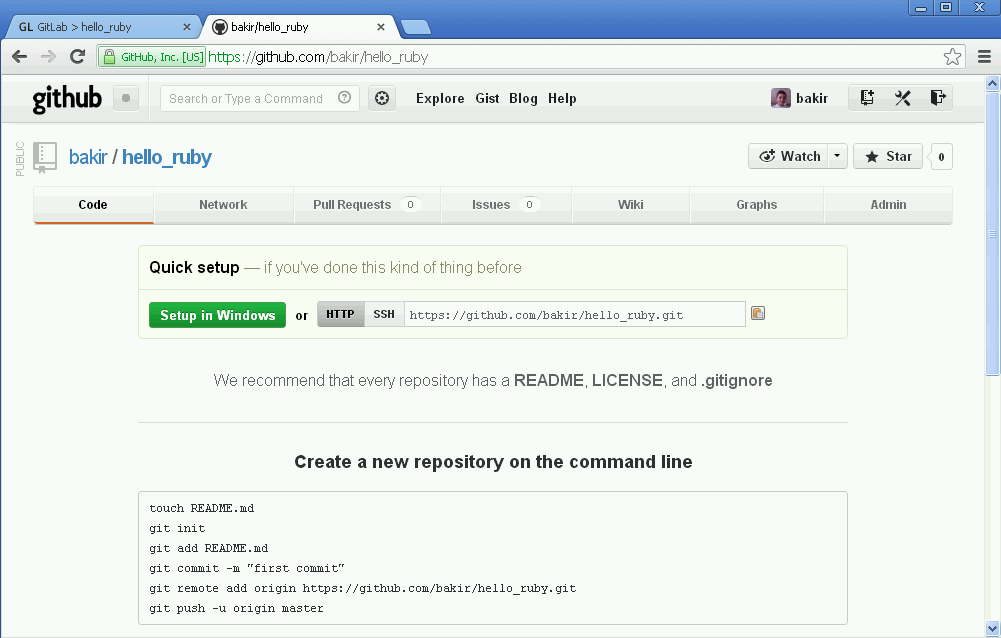
\includegraphics[width=15cm]{img/github_new_repos_2.png}
\caption{Github novi repozitorij / 2}
\end{figure}

\begin{figure}[H]
\centering
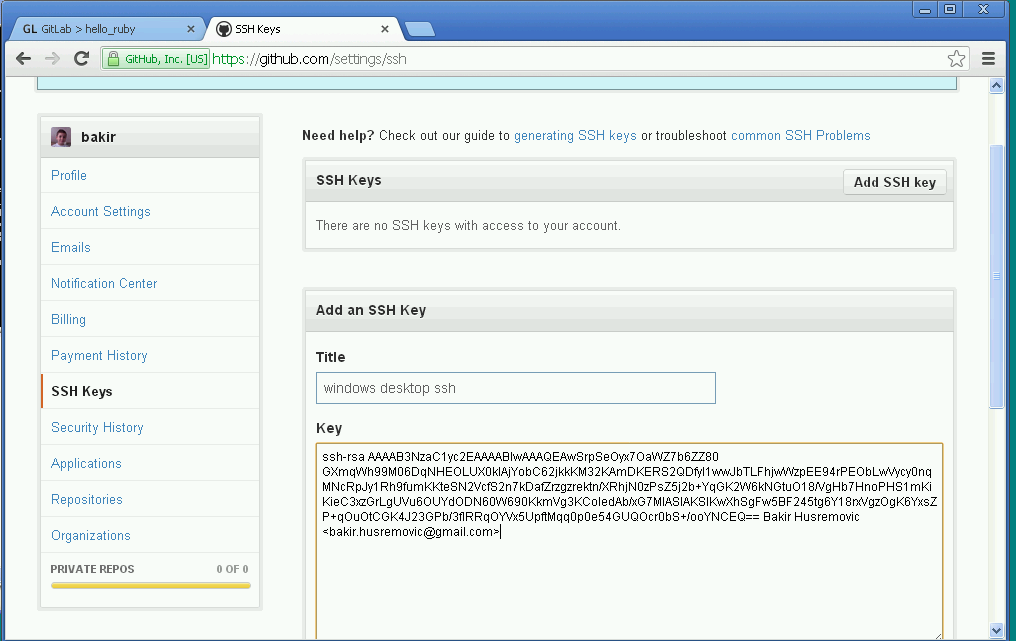
\includegraphics[width=15cm]{img/github_ssh_profile.png}
\caption{Github ssh profil}
\end{figure}

\begin{figure}[H]
\centering
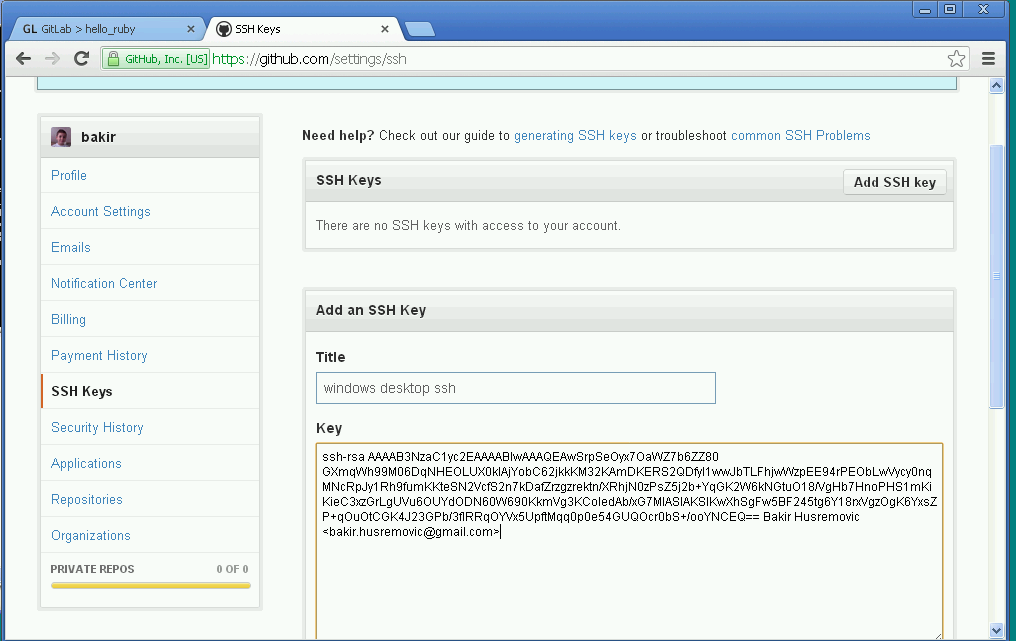
\includegraphics[width=15cm]{img/github_ssh_profile.png}
\caption{Github ssh profil /2}
\end{figure}

\begin{figure}[H]
\centering
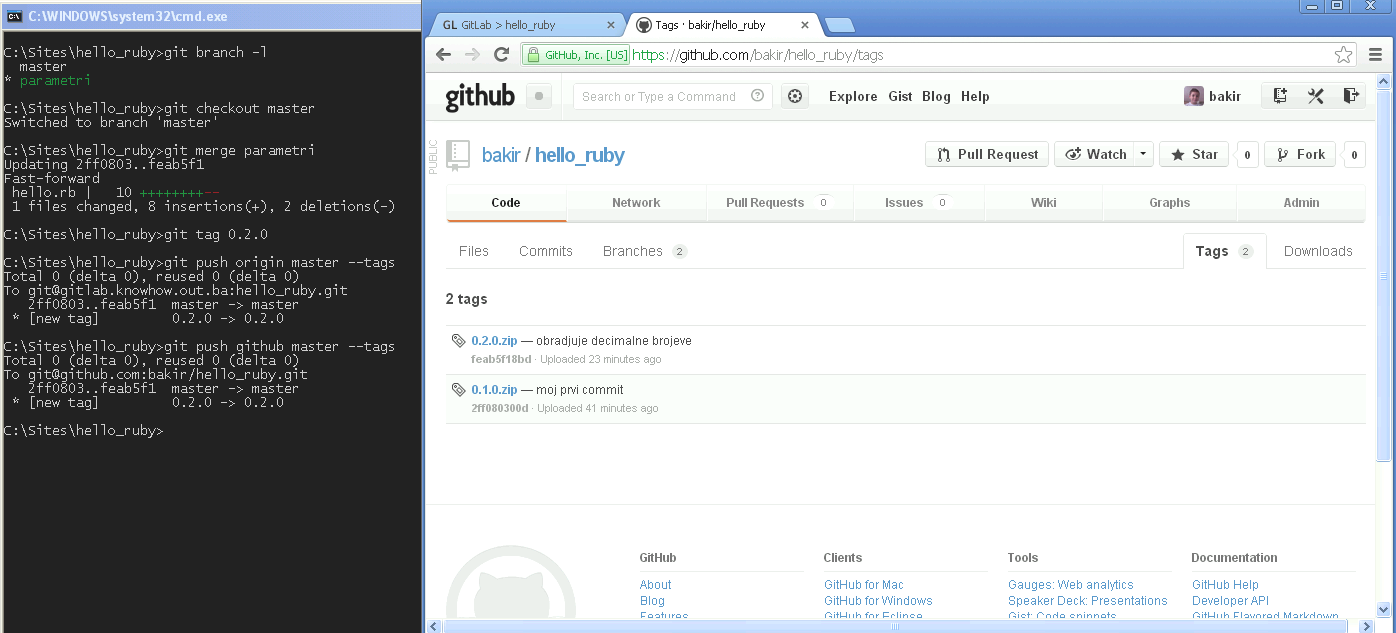
\includegraphics[width=16cm]{img/github_new_tag.png}
\caption{Github - novi tag}
\end{figure}

\begin{figure}[H]
\centering
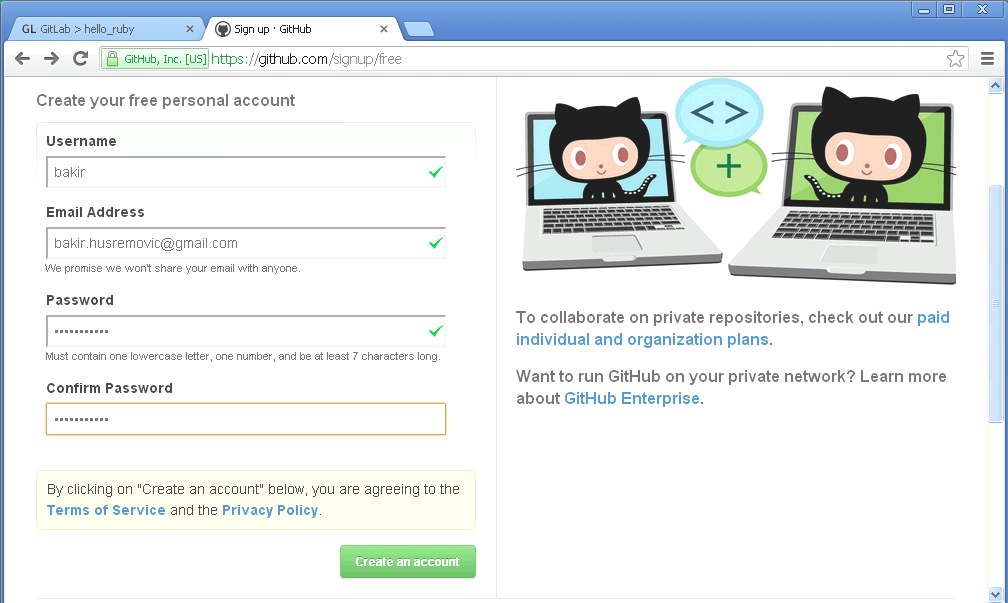
\includegraphics[width=15cm]{img/github_prijava.png}
\caption{Github prijava}
\end{figure}

\section{Branches}

\begin{figure}[H]
\centering
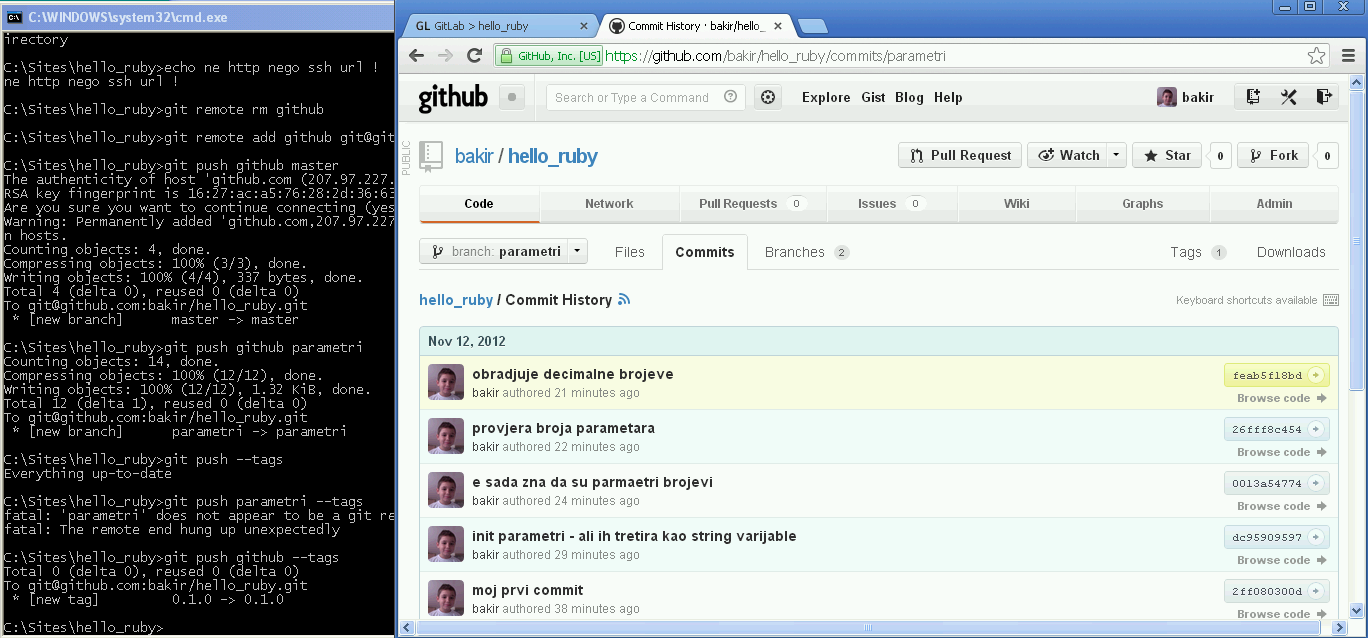
\includegraphics[width=15cm]{img/github_push_branches_and_tags.png}
\caption{Pošalji sve branchove i tag-ove na github repozitorij}
\end{figure}


\section{Compare}

\begin{figure}[H]
\centering
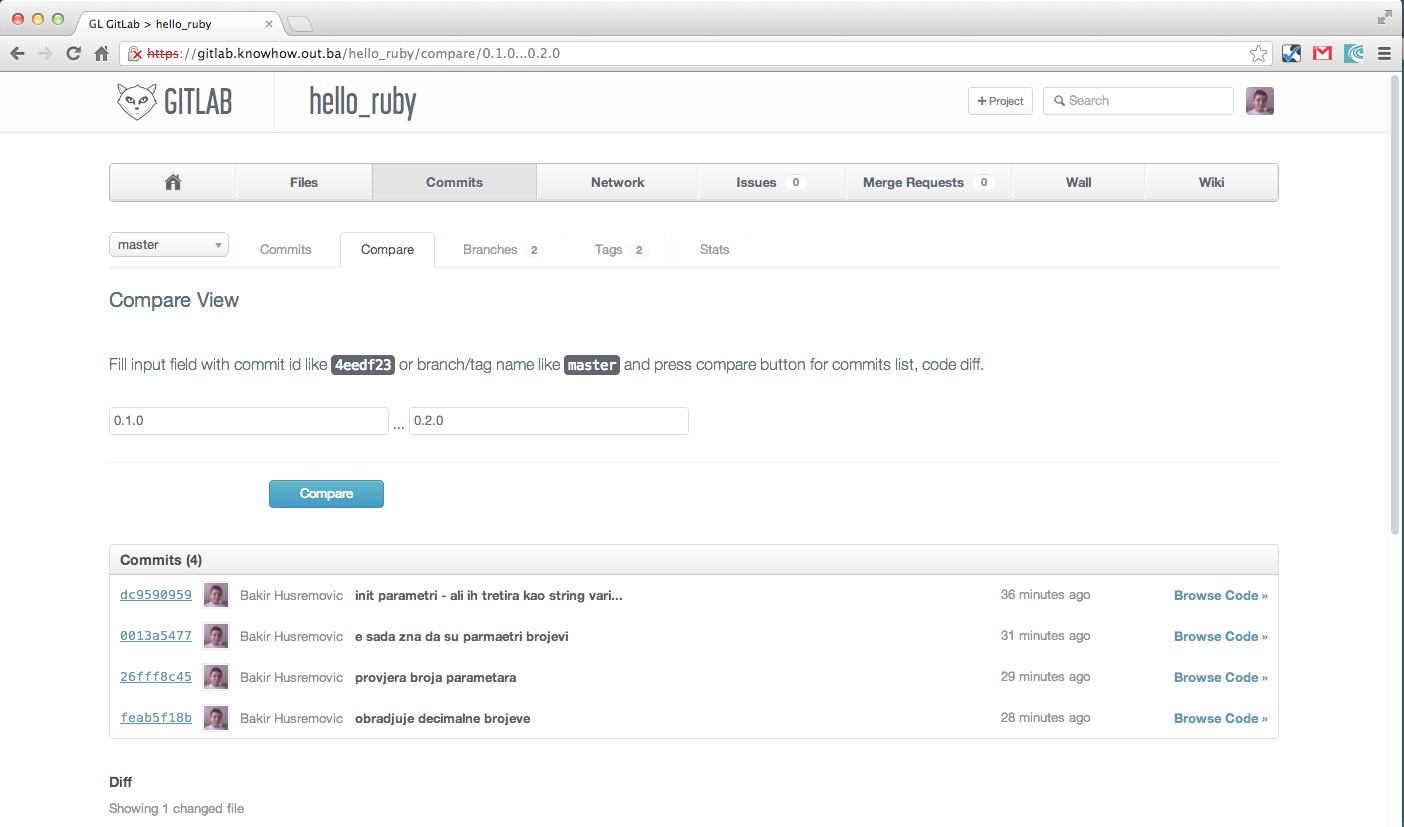
\includegraphics[width=15cm]{img/gitlab_compare.png}
\caption{Gitlab uporedi dvije verzije}
\end{figure}


\begin{figure}[H]
\centering
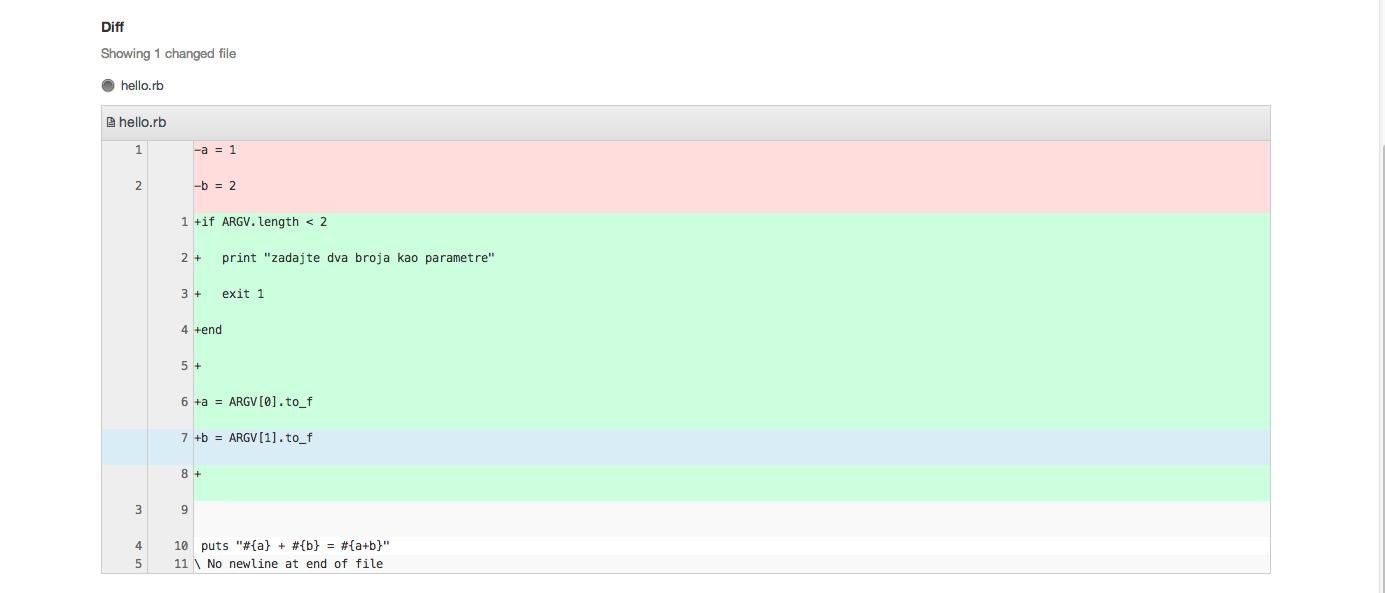
\includegraphics[width=15cm]{img/gitlab_compare_2.png}
\caption{Gitlab uporedi dvije verzije /2}
\end{figure}


\section{Notifikacija}

\begin{figure}[H]
\centering
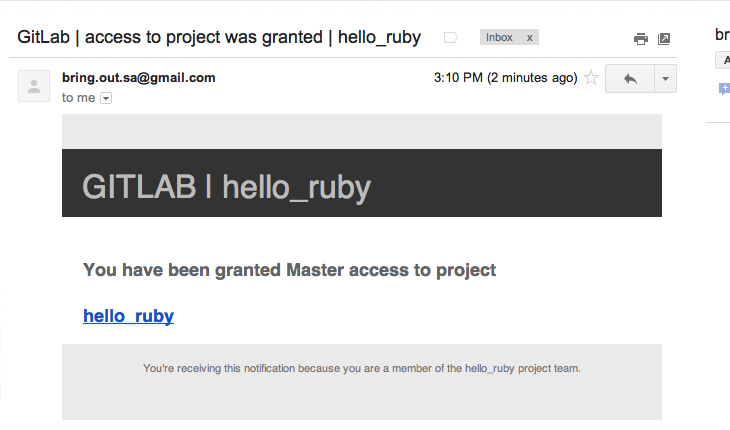
\includegraphics[width=15cm]{img/gitlab_email_notification.png}
\caption{Gitlab email notifikacija}
\end{figure}


\section{Commit}

\begin{figure}[H]
\centering
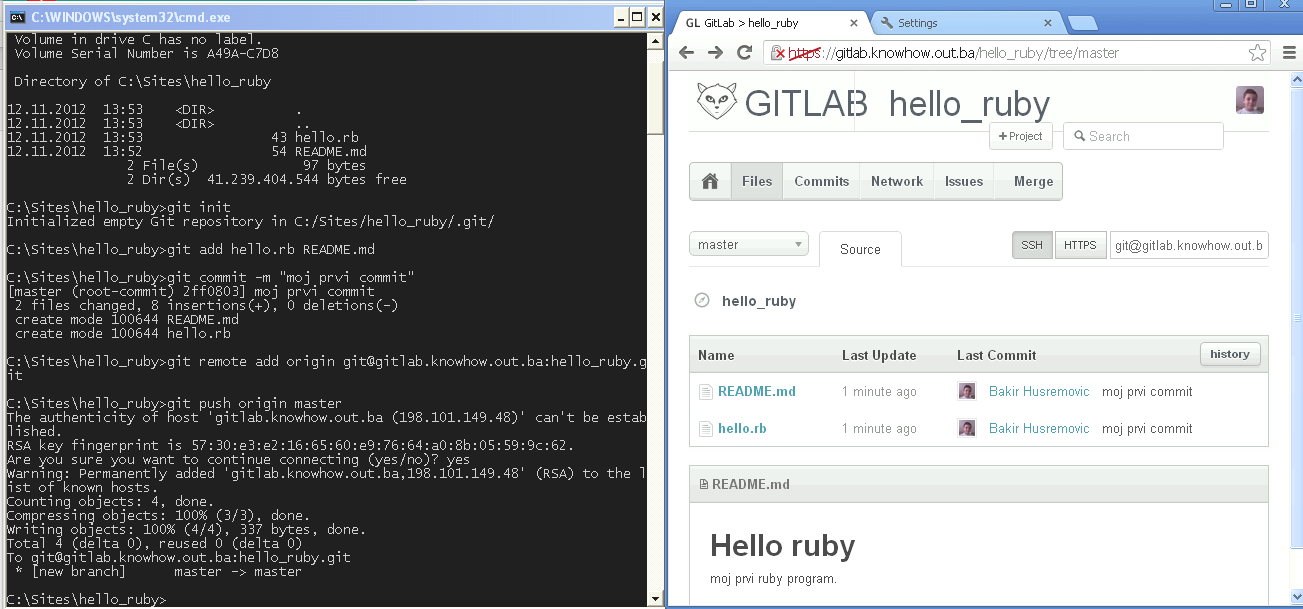
\includegraphics[width=15cm]{img/gitlab_first_commit.png}
\caption{Gitlab prvi commit}
\end{figure}


\begin{figure}[H]
\centering
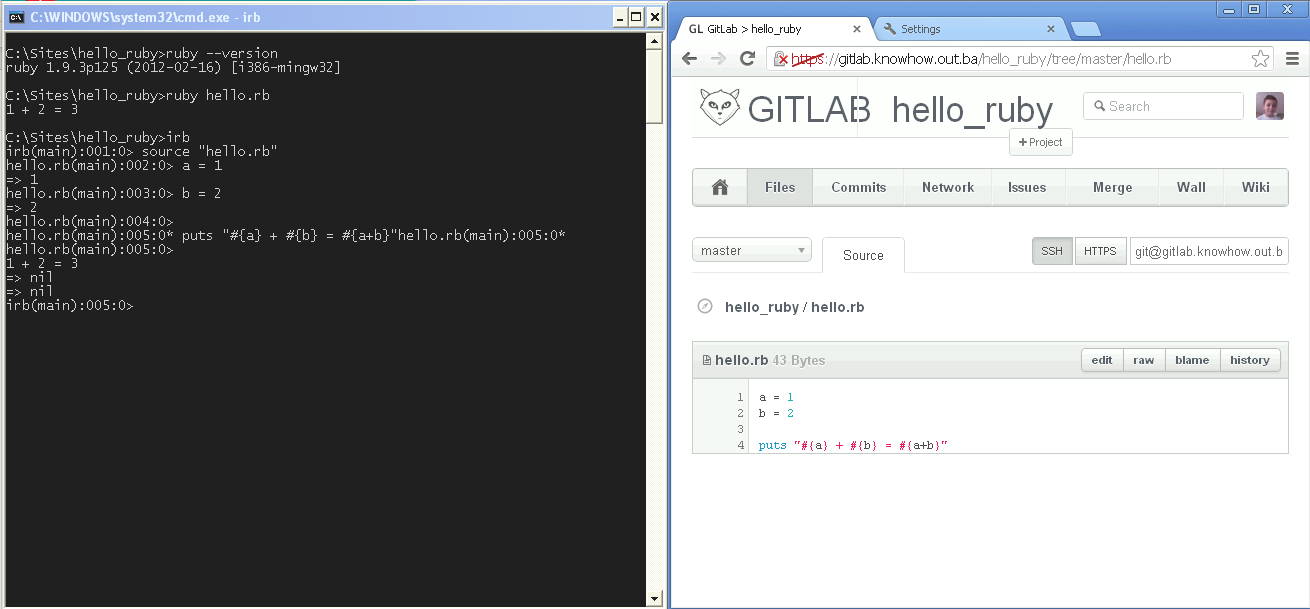
\includegraphics[width=15cm]{img/gitlab_first_commit_2.png}
\caption{Gitlab prvi commit /2}
\end{figure}

\section{Merge}

\begin{figure}[H]
\centering
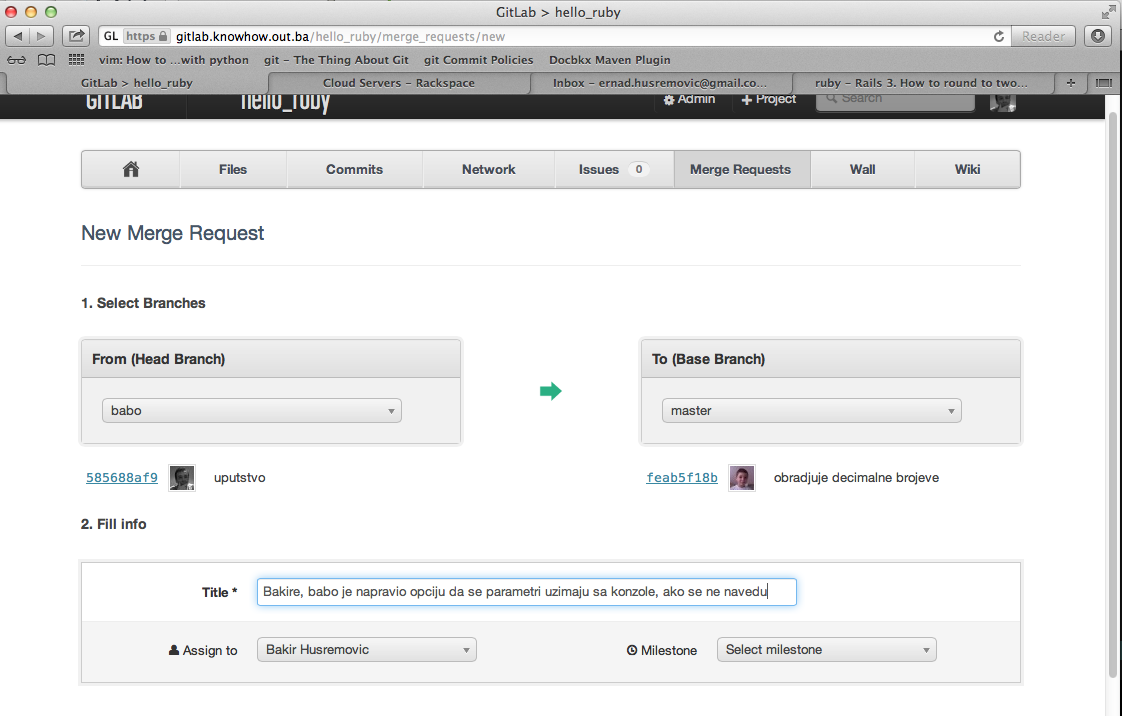
\includegraphics[width=15cm]{img/gitlab_merge_request.png}
\caption{Gitlab merge request}
\end{figure}


\begin{figure}[H]
\centering
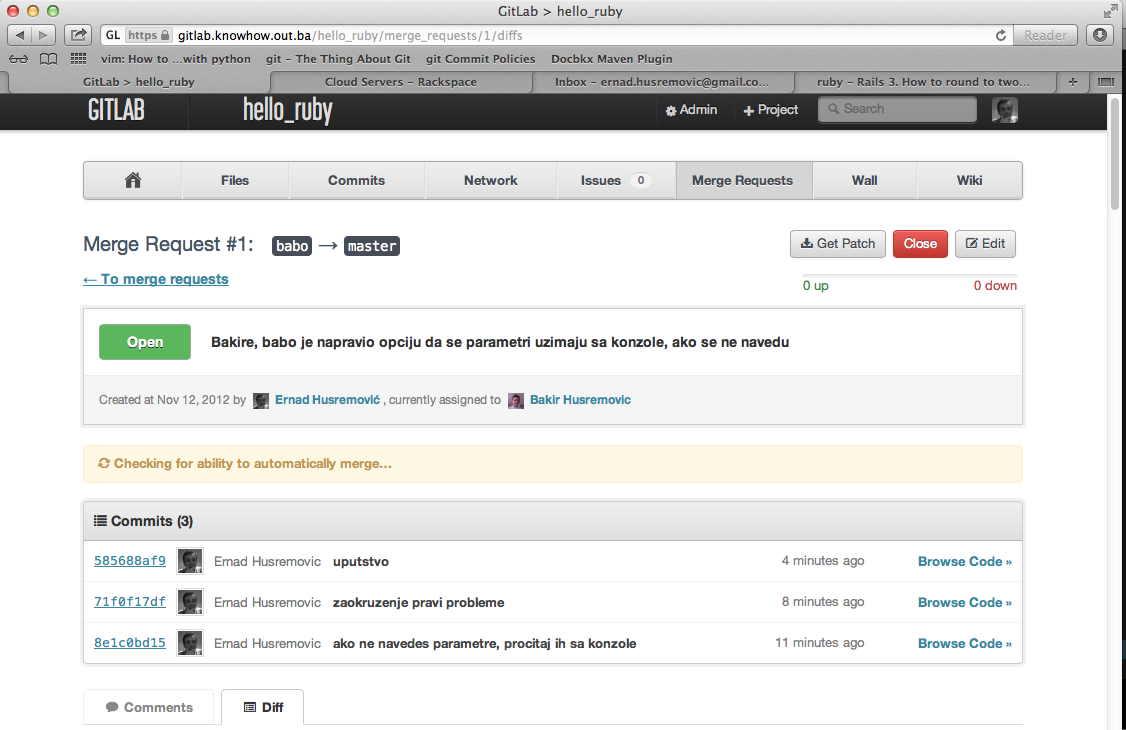
\includegraphics[width=15cm]{img/gitlab_merge_request_2.png}
\caption{Gitlab merge request /2}
\end{figure}

\begin{figure}[H]
\centering
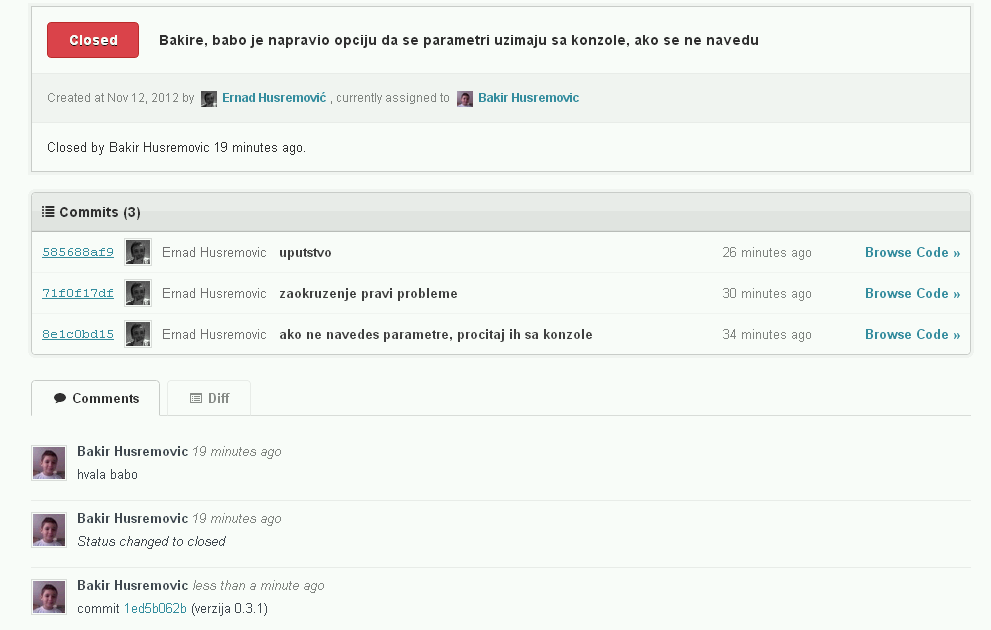
\includegraphics[width=15cm]{img/gitlab_merge_request_answer.png}
\caption{Gitlab merge request answer}
\end{figure}

\begin{figure}[H]
\centering
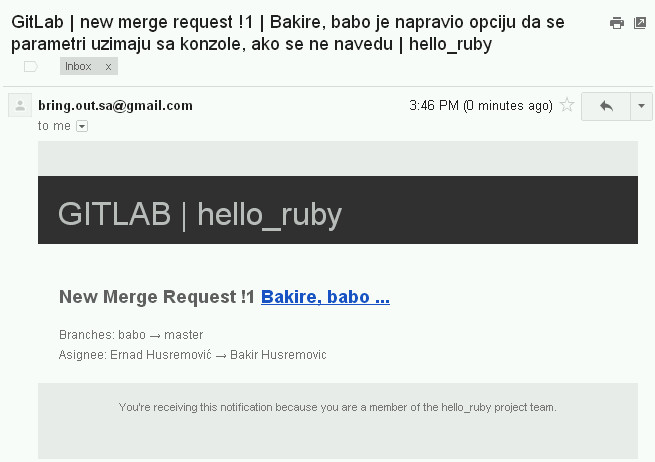
\includegraphics[width=15cm]{img/gitlab_merge_request_email_notification.png}
\caption{Gitlab merge request email notification}
\end{figure}


\section{GitlabHQ}

\begin{figure}[H]
\centering
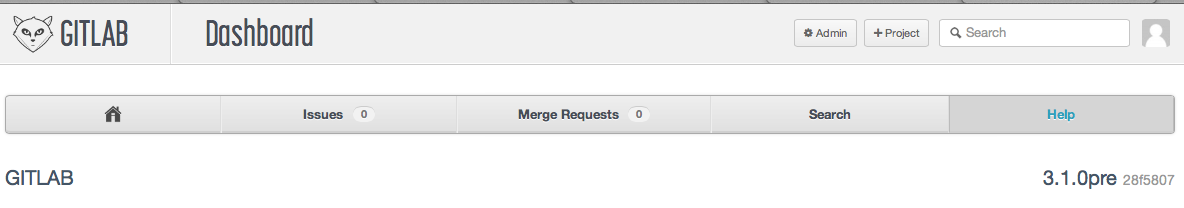
\includegraphics[width=15cm]{img/gitlab_hernad_310_after_merge.png}
\caption{Gitlabhq nakon `merge' operacije sa `upstream' projektom}
\end{figure}

\begin{figure}[H]
\centering
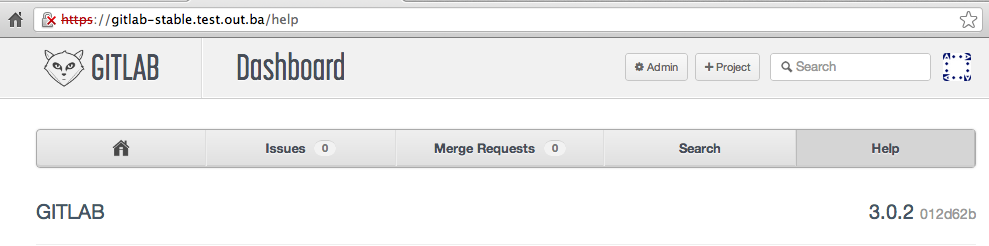
\includegraphics[width=15cm]{img/gitlab_stable_3.0.2.png}
\caption{Gitlabhq - stable 3.0.2}
\end{figure}


\begin{figure}[H]
\centering
\includegraphics[width=15cm]{img/gitlabhq_3.0.3.png}
\caption{Gitlabhq - 3.0.3}
\end{figure}



\subsection{Gitlabhq merge from upstream}

gitlabhq\$ git fetch gitlabhq

\begin{lstlisting}
remote: Counting objects: 570, done.
remote: Compressing objects: 100\% (174/174), done.
remote: Total 342 (delta 262), reused 237 (delta 165)
Receiving objects: 100\% (342/342), 43.70 KiB, done.
Resolving deltas: 100\% (262/262), completed with 122 local objects.
From git://github.com/gitlabhq/gitlabhq
   dd4d124..3c7806c  master     -> gitlabhq/master
\end{lstlisting}


gitlabhq\$ git branch -l

\begin{lstlisting}
* master
\end{lstlisting}


gitlabhq\$ git commit -a

\begin{lstlisting}
[master 9bacff4] http://www.quora.com/Ruby-on-Rails/What-is-schema-rb-in-rails-project
 1 file changed, 19 insertions(+), 19 deletions(-)
\end{lstlisting}



gitlabhq\$ git diff HEAD\^1 HEAD

\begin{lstlisting}
diff --git a/db/schema.rb b/db/schema.rb
index 51ab207..19eb8eb 100644
--- a/db/schema.rb
+++ b/db/schema.rb
@@ -69,8 +69,8 @@ ActiveRecord::Schema.define(:version => 20121026114600) do
     t.boolean  "closed",                              :default => false, :null => false
     t.datetime "created_at",                                             :null => false
     t.datetime "updated_at",                                             :null => false
-    t.text     "st_commits",    :limit => 2147483647
-    t.text     "st_diffs",      :limit => 2147483647
+    t.text     "st_commits",    :limit => 4294967295

  ...

     t.integer  "project_id"
     t.string   "attachment"
     t.string   "line_code"
@@ -156,30 +156,30 @@ ActiveRecord::Schema.define(:version => 20121026114600) do
   end
 
   create_table "users", :force => true do |t|
\end{lstlisting}


gitlabhq\$ git merge gitlabhq/master

\begin{lstlisting}
Removing lib/gitlab/encode.rb
Removing gitlab
Auto-merging doc/development.md
Removing Procfile.production
Merge made by the recursive strategy
 .travis.yml                                        |    2 +-
 CHANGELOG                                          |    2 +-
 Gemfile                                            |    4 +-
 Gemfile.lock                                       |   12 +++-
 Procfile.production                                |    2 -
 VERSION                                            |    2 +-
 app/assets/images/event_filter_comments.png        |  Bin 0 -> 750 bytes
 app/assets/images/event_filter_merged.png          |  Bin 0 -> 463 bytes
 app/assets/images/event_filter_push.png            |  Bin 0 -> 632 bytes
 
 ...

 app/controllers/application_controller.rb          |    9 +++
 app/controllers/blob_controller.rb                 |   10 +--
 app/controllers/dashboard_controller.rb            |   11 ++-
 app/controllers/profile_controller.rb              |    2 +-

 ...

 app/views/blame/show.html.haml                     |    4 +-
 app/views/commits/_commit.html.haml                |    4 +-
 app/views/commits/_head.html.haml                  |    5 ++
 app/views/dashboard/index.html.haml                |    9 ++-
 
 ... 
 
 delete mode 100644 Procfile.production
 create mode 100644 app/assets/images/event_filter_comments.png
 create mode 100644 app/assets/images/event_filter_merged.png
 create mode 100644 app/assets/images/event_filter_push.png
 ...
 delete mode 100644 lib/gitlab/encode.rb
 create mode 100644 lib/gitlab/git_stats.rb
 create mode 100644 vendor/assets/javascripts/g.bar-min.js
 create mode 100644 vendor/assets/javascripts/g.raphael-min.js
\end{lstlisting}



gitlabhq\$ git push origin master

\begin{lstlisting}
Counting objects: 581, done.
Delta compression using up to 8 threads.
Compressing objects: 100\% (85/85), done.
Writing objects: 100\% (350/350), 45.00 KiB, done.
Total 350 (delta 267), reused 342 (delta 262)
To git@github.com:hernad/gitlabhq.git
   038ac96..28f5807  master -> master

\end{lstlisting}



%\begin{center}
%\emph{\large{Freedom to create, distribute, and use open source software (OSS).}}
%\end{center}

\chapter {Gitlab}
\vspace*{-0.7cm}

\section{Source control}

\section{Issues}

\section{Wiki}

\chapter{Zaključak}

.

% -------------------------------------------------
\bibliography{literatura}
\bibliographystyle{fit}

% -------------------------------------------------
\appendix

\chapter{Instalacija}
\vspace*{-0.7cm}
\setlength{\parindent}{0cm}
%\setlength{\parindent}{default}

\chapter{Software toolset}
\begin{enumerate}
  \item Mac OS X 10.8.2
  \item mvim, vim tekst editor ver 7.3
  \item MacTex (TeX Live 2012)
\end{enumerate}

\chapter{Software repozitoriji}

\begin{itemize}
  \item Agilni developerski environment  \url{https://github.com/hernad/atile\_dev\_env}

\end{itemize}

\end{document}
